\documentclass[a4paper]{article}
\usepackage[margin=1in]{geometry}
\usepackage{graphicx}
\usepackage{enumitem}
\usepackage{listings}
\usepackage[utf8x]{inputenc}
\usepackage[spanish,es-tabla]{babel}
\usepackage{amssymb,amsmath,amsthm,amsfonts}
\usepackage{calc}
\usepackage{subcaption}
\usepackage{textcomp}
\usepackage{gensymb}
\usepackage{natbib}
\usepackage{parskip}
\usepackage{fancyhdr}
\usepackage{vmargin}
\usepackage{pdfpages}
\usepackage{pgfplots}
\usepackage{multicol}
\usepackage{multirow}
\usepackage{array}
\usepackage{booktabs}
\usepackage{wrapfig} 
\usepackage{hyperref}
\usepackage{tikz}
\usepackage{makecell}

\usepackage[table,xcdraw]{xcolor}
\usepackage{tabularx}


\hypersetup{
    colorlinks=true,
    linkcolor=black,
    filecolor=magenta,      
    urlcolor=blue,
    }

\urlstyle{same}

\lstdefinestyle{Golang}{ % add your own preferences
    frame=single,
    basicstyle=\footnotesize,\ttfamily,breaklines=true
    keywordstyle=\color{red},
    numbers=left,
    numbersep=5pt,
    showstringspaces=false, 
    stringstyle=\color{blue},
    commentstyle=\color{green},
    tabsize=4,
    language=Go
}


\usetikzlibrary{datavisualization}
\newcolumntype{P}[1]{>{\centering\arraybackslash}p{#1}}
\newcolumntype{M}[1]{>{\centering\arraybackslash}m{#1}}

\pgfplotsset{compat=1.12}
\usepgfplotslibrary{fillbetween}
\usetikzlibrary{patterns}

% \newcommand{\gettikzxy}[3]{%
%   \tikz@scan@one@point\pgfutil@firstofone#1\relax
%   \global\edef#2{\the\pgf@x}%
%   \global\edef#3{\the\pgf@y}%
% }
% \newcommand{\gettikzcoordinates}[2]{%
%   \tikz@scan@one@point\pgfutil@firstofone#1\relax
%   \pgfmathsetmacro{\myx}{round(0.99626*\the\pgf@x/0.0283465)/1000}
%   \pgfmathsetmacro{\myy}{round(0.99626*\the\pgf@y/0.0283465)/1000}
%   \global\edef#2{(\myx,\myy)}%
% }
\makeatother

%\setmarginsrb{3 cm}{2.5 cm}{3 cm}{2.5 cm}{0.5 cm}{1 cm}{0.5 cm}{1 cm}
\title{Estudio del Flujo de control Secuencia Paralelo en Go}					                                % Titulo documento
\author{José Pinto Villamar}				                                                                              	% Autor
\date{\today}					                                                                        	% Fecha

% \makeatletter
% \let\thetitle\@title
% \let\theauthor\@author
% \let\thedate\@date
% \makeatother

\pagestyle{fancy}
\fancyhf{}
\rhead{}                                                                                        % Encabezado pagina DER
\lhead{Estudio del Flujo de control Secuencia / Paralelo en Go}                                                                        % Encabezado pagina IZQ
\cfoot{\thepage}

\newcommand{\HRule}{\rule{\linewidth}{0.5mm}}
\newcommand{\HRulee}{\rule{\linewidth}{0.2mm}}

\begin{document}
\graphicspath{{./images/}}

%%%%%%%%%%%%%%%%%%%%%%%%%%%%%%%%%%%%%%%%%%%%%%%%%%%%%%%%%%%%%%%%%%%%%%%%%%%%%%%%%%%%%%%%%
% incluir una portada de la uni en PDF
%\includepdf[pages=-, scale=1, offset=23mm -20mm]{tapa_informe.pdf}
%%%%%%%%%%%%%%%%%%%%%%%%%%%%%%%%%%%%%%%%%%%%%%%%%%%%%%%%%%%%%%%%%%%%%%%%%%%%%%%%%%%%%%%%

\begin{titlepage}
    \centering
    
    % \textsc{\LARGE Universidad La Salle}\\[0.2cm]
    \textsc{\Large Facultad de Ingenierías y Matemáticas}\\[0.2cm]
    \textsc{\Large Carrera Profesional de Ingeniería de Software}\\[0.2cm]
    \textsc{\Large Computación Distribuida y Paralela}\\[0.5cm]
    
    \centering
        \vspace*{0.0 cm}
        \begin{figure}
            \centering
            \hspace{1cm}
            
\includegraphics[height = 65px]{logo-la-salle.pdf}
            % \hspace{5cm}
            % \includegraphics[height = 100px]{dimec.png}
        \end{figure}
    
    \HRule{} \\[0.5cm]
    { \LARGE \bfseries Estudio del Flujo de control Secuencia / Paralelo en Go}\\[0.3cm]
    \HRule{} \\[0.5cm]
    
    
\includegraphics[width = 0.6\textwidth]{Go_Logo_Blue.pdf}\\[0.5cm]

    \Large \emph{Docente:}\\
    Richart Smith \textsc{Escobedo Quispe}\\
    \href{mailto:r.escobedo@ulasalle.edu.pe}{r.escobedo@ulasalle.edu.pe}\\[0.5cm]
    
    \Large \emph{Desarrollado por:}\\
    José Alfredo \textsc{Pinto Villamar}\\
    \href{mailto:jpintov@ulasalle.edu.pe}{jpintov@ulasalle.edu.pe}\\[0.5cm]
    
    {\large \today}\\[2cm]
    
    \end{titlepage}
%%%%%%%%%%%%%%%%%%%%%%%%%%%%%%%%%%%%%%%%%%%

% \tableofcontents
% \pagebreak

% \listoffigures
% \listoftables
% \pagebreak

%============================================


\section{Introducción}
En este trabajo se realizaron ensayos de los tiempos de ejecución para hallar el área
de una función matemática, usando así la regla del trapecio.

En el cálculo, la regla trapezoidal también conocida como la regla del trapecio es una
técnica de aproximación numérica de la integral definida.

\begin{equation}
\int_{a}^{b} f(x) dx
\end{equation}

La regla trapezoidal funciona aproximando la región bajo el gráfico de la función $f(x)$
como un trapecio y calculando su área.

\begin{equation}
\int_{a}^{b} f(x) dx \approx (b-a) \cdot \tfrac{1}{2}(f(a) + f(b)).
\end{equation}

La regla del trapecio puede ser vista como el resultado obtenido al promediar los valores
de la función en los extremos del intervalo $a$ y $b$. La regla del trapecio es un caso
especial de la regla de Simpson, que es una regla de integración numérica más general.
Incluso, la integral se puede aproximar aún mejor dividiendo el intervalo de integración
aplicando la regla del trapecio a cada subintervalo, y sumando los resultados.
En la práctica sería así\nocite{cruz2002sharp}:

Sea: $\{x_k\}$ una partición de $[a,b]$ tal que $a = x_0 < x_1 < \cdots < x_{N-1} < x_N = b$
y $\Delta{x_k}$ es la longitud de $k$-ésimo subintervalo (es decir, $\Delta{x_k} = x_{k+1} - x_k$), entonces:

\begin{equation}
\int_{a}^{b} f(x) dx \approx \sum_{k=1}^{N} \frac{f(x_{k-1}) + f(x_{k})}{2}  \Delta{x_k} 
\end{equation}

Cuando la partición tiene un número par de subintervalos, la regla del trapecio es exacta
y podemos decir que todos los $\Delta{x_k}$ tienen el mismo valor $\Delta{x}$, entonces
la fórmula se puede simplificar para calcular la eficiencia factorizando $\Delta{x}$ \nocite{rahman1990characterization}:

\begin{equation}
\int_{a}^{b} f(x) dx \approx \frac{\Delta {x}}{2} (f(x_0) + 2f(x_1) + 2f(x_2) + \cdots + 2f(x_{N-1}) + f(x_N))
\end{equation}



\begin{equation}
\int_{a}^{b} f(x) dx \approx \frac{\Delta{x}}{2} \sum_{k=1}^{N} (f(x_{k-1}) + f(x_{k}))
\end{equation}


\section{Ejecuciones en Sequencial}

\subsection{Código en Go}
%% import code from a folder
\begin{lstlisting}[style=Golang]
  package main

  import (
    "fmt"
    "math"
    "strings"
    "text/template"
    "time"
  )
\end{lstlisting}
Aquí simplemente se importan las librerías necesarias para el desarrollo del código.
\pagebreak

\begin{lstlisting}[style=Golang, firstnumber=11]
  func format(s string, v interface{}) string {
    t, b := new(template.Template), new(strings.Builder)
    template.Must(t.Parse(s)).Execute(b, v)
    return b.String()
  }
\end{lstlisting}
Esta función \texttt{format} me sirve para darle formato a mis \texttt{outputs} de la consola. \\
\\

\begin{lstlisting}[style=Golang, firstnumber=17]
  func TrapezoidRule(f func(float64) float64, a, b float64, n int) float64 {
    h := (b - a) / float64(n) sum := 0.5 * (f(a) + f(b))
    for i := 1; i < n; i++ {
      sum += f(a + float64(i)*h)
      }  
    return sum * h
    }
\end{lstlisting}
Esta es la parte más importante, y es dónde se aplica la regla del trapecio.
Yo la hice un poco diferente a lo planteando en clase porque pienso que sin
utilizar arrays puede llegar a ser más eficiente. En este caso, uso un bucle for
que va desde 1 hasta n, y en cada iteración se va sumando el valor de la función
en el punto $x_i$ al valor de la suma. Y retorno el valor de la suma multiplicado
por el valor de $h$. \\ \\

\begin{lstlisting}[style=Golang, firstnumber=26]
  f := func(x float64) float64 {
		return ((math.Pow(x, 2) + 1) / 2)
	}

  n := 1
	start := time.Now()
	elapsed := time.Since(start).Nanoseconds()
	result := TrapezoidRule(f, 5, 20, n)
	area := format("Area: {{ . }}.", result)
	fmt.Println(area)
	time := format("Time: {{ . }} in ns.", elapsed)
	fmt.Println(time)
	fmt.Println()
  
\end{lstlisting}
Y como parte final agregamos el \texttt{main} los \texttt{prints} para que podamos ver los resultados.
También podemos ir cambiando el valor de $n$ el cual es el número de trapecios que se 
van a utilizar.


\section{Paralelo}
\subsection{Código en Go}

\begin{lstlisting}[style=Golang]
  package main

  import (
    "fmt"
    "sync"
    "time"
  )
\end{lstlisting}
En este caso, importamos la librería \texttt{sync} para poder utilizar 
\texttt{waitgroup}.

\begin{lstlisting}[style=Golang,firstnumber=9]
  var times time.Duration
  var wg sync.WaitGroup
\end{lstlisting}
En esta parte se declaran las variables que se van a utilizar para hacer
el cálculo en paralelo.\\
\\

\begin{lstlisting}[style=Golang,firstnumber=12]
  type Trapezoid struct {
    f func(float64) float64
    a float64
    b float64
    n int
  }

\end{lstlisting}
En este caso he creado una clase para hacerlo más sencillo al momenento de ingresar
los datos.\\
\\

\begin{lstlisting}[style=Golang,firstnumber=19]
  func (t *Trapezoid) TrapezoidRule() float64 {
    h := (t.b - t.a) / float64(t.n)
    sum := 0.5 * (t.f(t.a) + t.f(t.b))
    for i := 1; i < t.n; i++ {
      wg.Add(1)
      sum += t.f(t.a + float64(i)*h)
      wg.Done()
    }
    return sum * h
  }
  
\end{lstlisting}
Atención a la la línea 23, donde se agrega un \texttt{waitgroup} para que el programa
espere a que se termine de ejecutar el bucle for. Y en la línea 25 acaba, y está listo para
volver a llamar función. \nocite{tu2019understanding}

\begin{lstlisting}[style=Golang, firstnumber=30]

  func main() {
    f := func(x float64) float64 {
      return ((x*x + 1) / 2)
    }
    t := Trapezoid{f, 5, 20, 10}
    start := time.Now()
    result := t.TrapezoidRule()
    elapsed := time.Since(start).Nanoseconds()
    defer fmt.Println(elapsed)
    area := fmt.Sprintf("Area: %v", result)
    fmt.Println(area)
    wg.Wait()
  
  
\end{lstlisting}
Y es aquí donde se llama a la función \texttt{TrapezoidRule} y se imprime el resultado.
Tenindo en cuenta que también se llamará a la función \texttt{Wait}, para ejecutar los procesos
en paralelo.

\section{Resultados}
% Please add the following required packages to your document preamble:
% \usepackage[table,xcdraw]{xcolor}
% If you use beamer only pass "xcolor=table" option, i.e. \documentclass[xcolor=table]{beamer}
Las siguientes gráficas son muestra de las pruebas que se hicieron.
Se realizó 10 pruebas en cada ciclo, es decir, en 1 trapecio, se realizaron
10 pruebas para sacar el promedio de tiempo. Y así sucesivamente. \\
\begin{figure}[H]
\centering
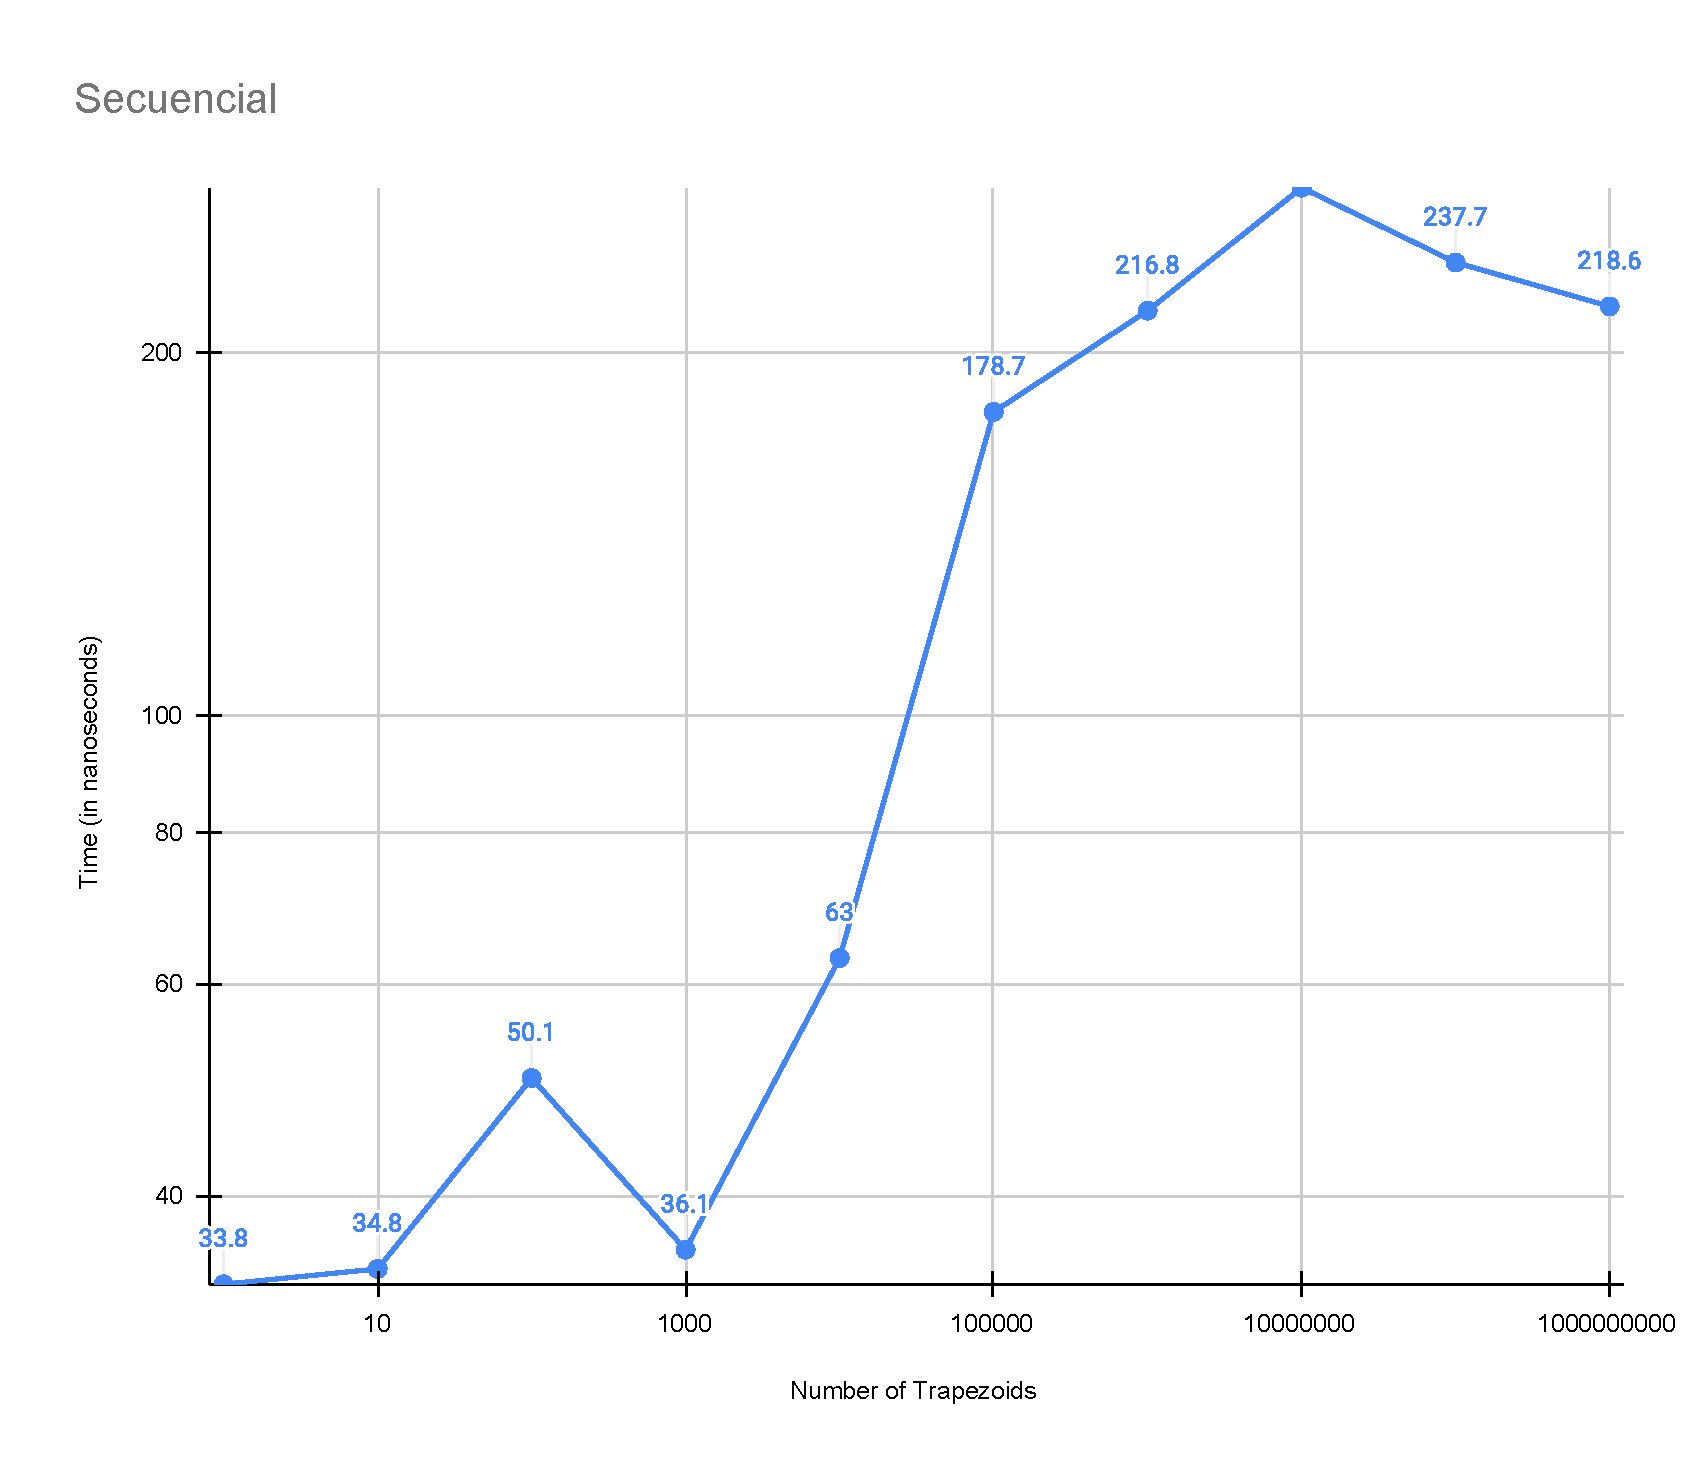
\includegraphics[width=0.7\textwidth]{Secuencial.pdf}
\caption{Tiempo de ejecución de la regla del trapecio en programación secuencial.}
\end{figure}

\begin{figure}[H]
\centering
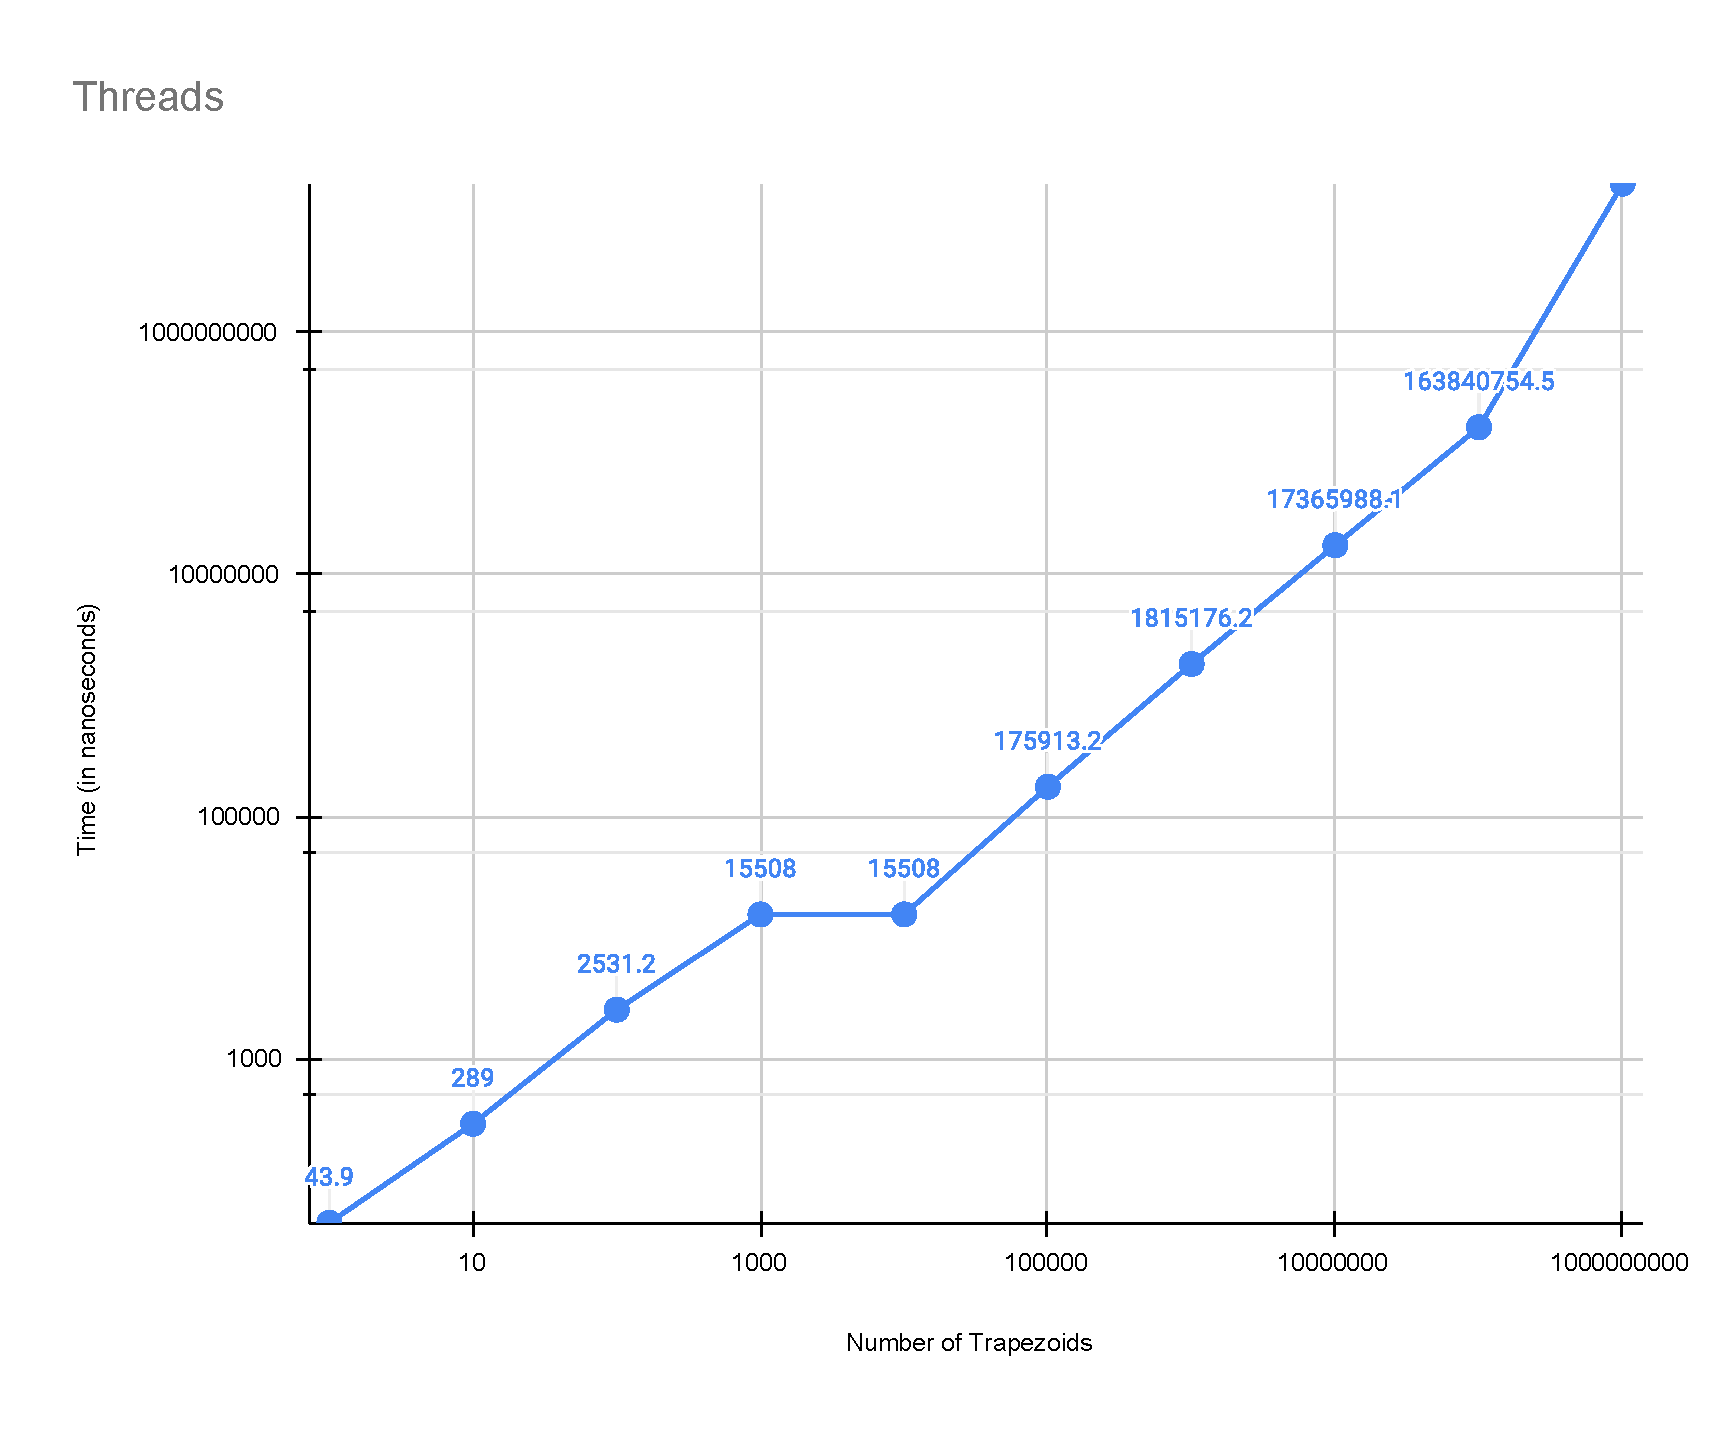
\includegraphics[width=0.7\textwidth]{Threads.pdf}
\caption{Tiempo de ejecución de la regla del trapecio en programación paralela.}
\end{figure}

\pagebreak

\section{Repositorio}
\begin{itemize}
\item \href{https://github.com/pintovillamar/computacion-distribuida-y-paralela/tree/main/tarea01-golang}{https://github.com/pintovillamar/computacion-distribuida-y-paralela/tree/main/tarea01-golang}
\end{itemize}


\bibliographystyle{ieeetr}
\bibliography{refs.bib}


\end{document}